\documentclass[UTF8]{beamer} 
\usepackage{ctex}
\usepackage{Sweave}
\usetheme{Boadilla} 
\usepackage{color} 
\usepackage{graphicx} 

\begin{document}

\title{R编程与进化分析} 
\subtitle{第三部分 进化树及系统发育比较分析}
\author{张金龙} 
\institute{jinlongzhang01@gmail.com}
\date{2016年5月9日 北京} 

\frame{\titlepage} 

\begin{frame}
\frametitle{目录}
\tableofcontents
\end{frame}


%%%%%%%%%%%%%%%%%%%%%%%%%%%%%%%%%%%%%%%%%%%%%%%%%%%%%%%%%%
%%%%%%%%%%%%%%%%%%%%%%%%%%%%%%%%%%%%%%%%%%%%%%%%%%%%%%%%%%
\section{进化树及其构建}

\begin{frame}
\frametitle{目录}
\tableofcontents[currentsection] 
\end{frame}


\frame{
    \frametitle{什么是进化树}
从DNA序列等推断出的物种系统发育关系, 用树状图表示, 即为进化树。 进化树是进行系统发育比较分析 Phylogenetic Comparative Methods的基础。
\begin{itemize}
\item 体现分类单元甚至个体的等级结构, 不一定能体现系统发育关系。 
\item 体现分类单元甚至个体的系统发育关系, 具有精确的枝长。
\item 体现分类单元之间的系统发育关系, 枝长以时间为单位。 
\end{itemize}
}

\frame{
    \frametitle{进化树的里程碑}
    \begin{itemize}
    \item 1859年, 达尔文引入了亲缘关系的树状图
    \item 十九世纪末, 海克尔用进化树表示物种之间的亲缘关系。
    \item 1964年, Cavalli-Sforza 和 Edwards提出了用简约法和极大似然法构建进化树。 
    \item Hennig 提出了分支理论 (Theory of cladistics)
    \item 1977年, Fitch将简约法应用到构建进化树中。
    \item 1978年, Felsenstein首次用极大似然法构建进化树
    \item 1996年, Rannala和杨子恒将贝叶斯推断引入到进化树的构建中。
    \end{itemize}
}

\frame{
    \frametitle{各种进化树}
      \begin{center}
     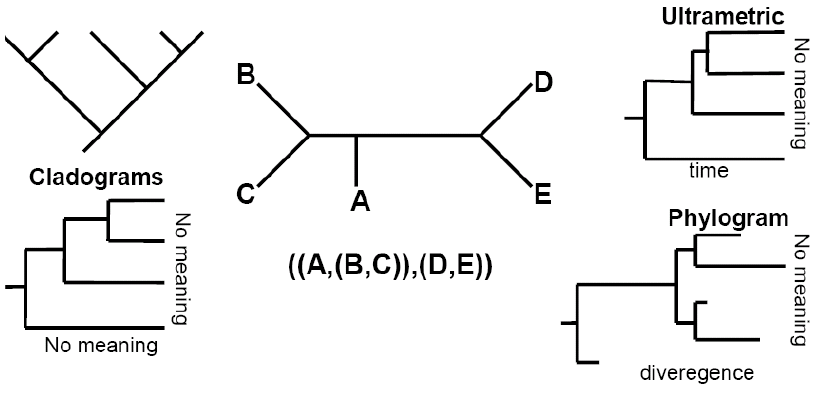
\includegraphics[height=2.5in]{phyo.png}\\
     \end{center}
}

\frame{
    \frametitle{Newick Format}
     \begin{center}
     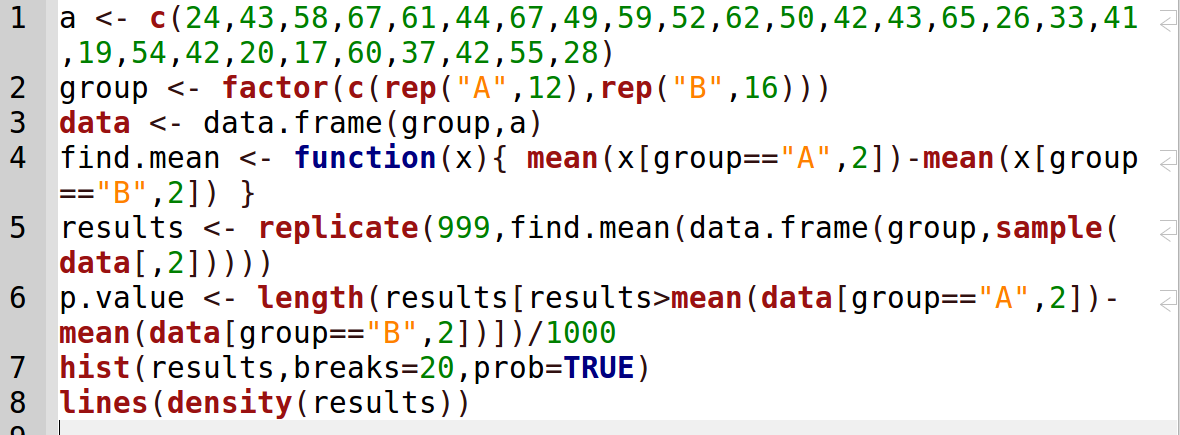
\includegraphics[height=2.2in]{Selection_061.png}\\
     \end{center}
     dopted by James Archie, William H. E. Day, Joseph Felsenstein, Wayne Maddison, Christopher Meacham, F. James Rohlf, and David Swofford, at two meetings in 1986, the second of which was at Newick's restaurant in Dover, New Hampshire, US. PHYLIP,RAxML等就用这种格式。 
}


\frame{
    \frametitle{Nexus格式 }
     \begin{center}
     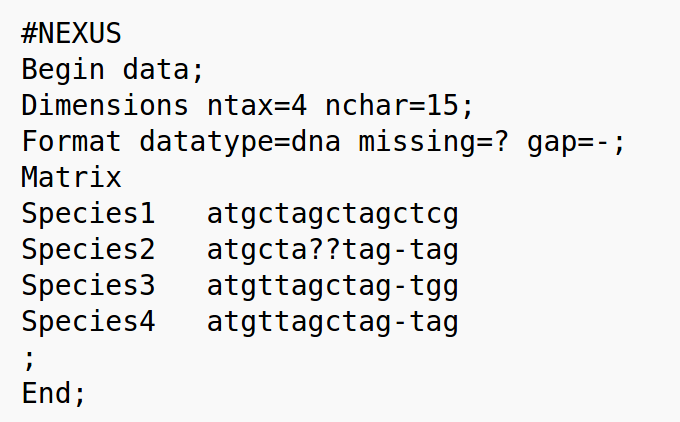
\includegraphics[height=2.2in]{Selection_063.png}\\
     \end{center}
     是Newick格式的升级版,可以增加多种blocks。BEAST,PAUP*, MrBayes, Mesquite,r8s等都使用该格式。  
}


\frame{
    \frametitle{其他格式 }
New Hampshire eXtended format (NHX) (http://home.cc.umanitoba.ca/~psgendb/doc/atv/NHX.pdf)\\
Jplace (http://journals.plos.org/plosone/article?id=10.1371/journal.pone.0031009)\\
}


\frame{
    \frametitle{重要概念: 等距树、有根树和外类群}
\begin{itemize}
\item 等距树 Ultrametric Tree: 每个末端分类单元都与根节点距离相同。  
\item 有根树 Rooted Tree: 探讨某类群系统发育关系时, 在该类群之外寻找的一个或者几个外类群。经过调整顺序后, 便于分析内部的系统发育关系。这样的进化树称为有根树。
\item 外类群 Outgroup:与研究的类群系统发育举例适中, 不能处在研究的类群中, 也不能太远。 
\end{itemize}
}

\frame{
    \frametitle{无根树和有根树以及外类群}
      \begin{center}
     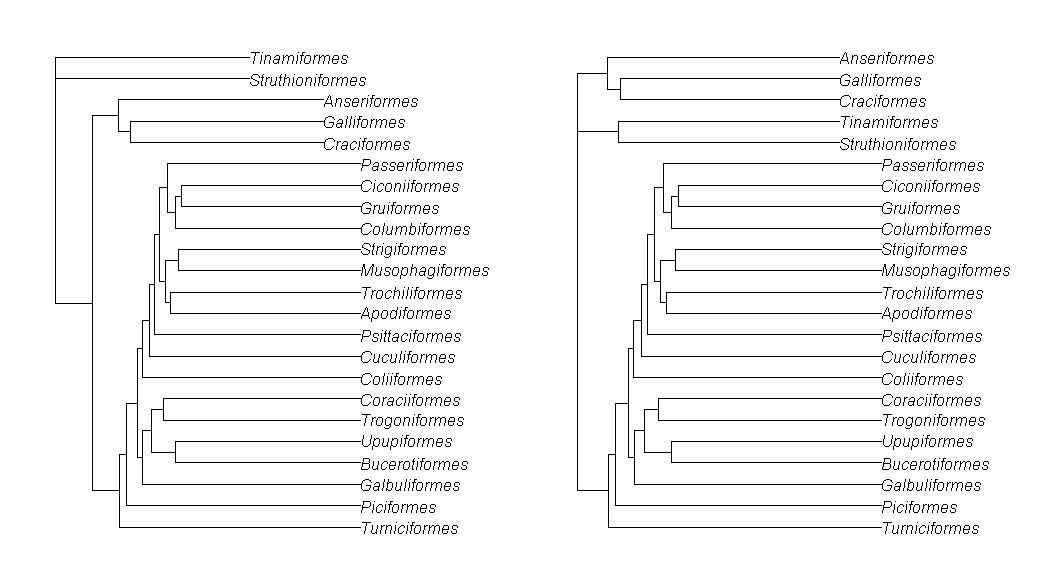
\includegraphics[height=2.5in]{phylo4.png}\\
     \end{center}
}
\frame{
    \frametitle{重要概念: 一致性树 Consensus Tree}
当获得多个进化树时, 可以对进化树内部节点的支持率进行汇总。 按照节点一致性的原则, 选出各进化树都支持的某节点的拓扑结构, 以及所支持的百分率, 称为节点支持率。  
}

\frame{
    \frametitle{重要概念: 二叉树, Singleton和Polytomies}

\begin{itemize}
\item 正常情况下, 每个节点下, 应该有两个子代。 这种进化树称为二叉树。
\item  若一个节点下, 只有一个节点, 称为 孤立节点 Singleton。
\item 若某一节点下, 有多个子代, 则生成如降落伞一样的多分枝结构。 
\end{itemize}
形成多分枝结构的原因: 物种数据缺失, 如建树的基因突变率很低, 无法反应出足够的系统发育距离。\\ 
用Phylomatic软件等生成的进化树, 常常包含 Singletons以及多分枝结构。\\

}

\frame{
    \frametitle{多分枝结构}
      \begin{center}
     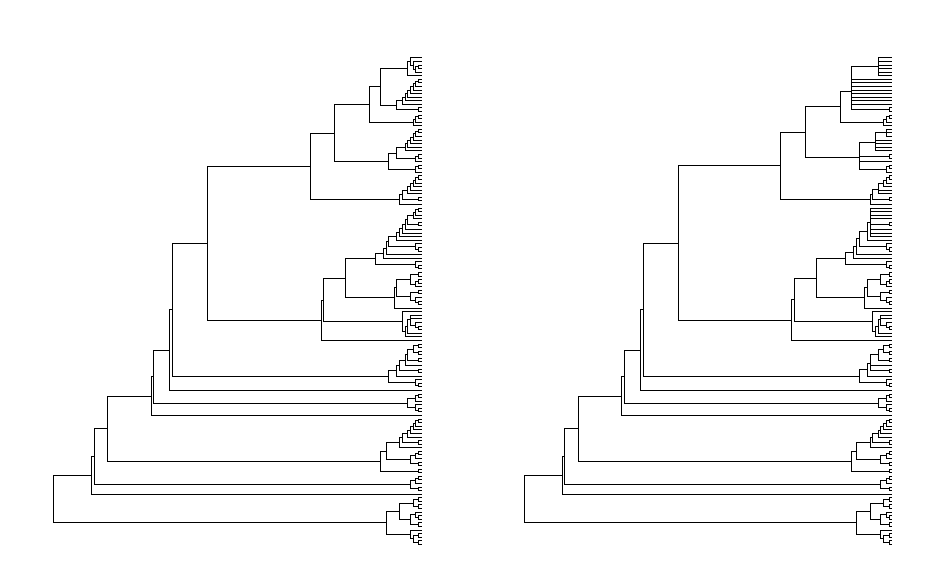
\includegraphics[height=2.5in]{phylo5.png}\\
     \end{center}
}

\frame{
    \frametitle{DNA序列}
DNA序列的获取\\
\begin{itemize}
\item 1. DNA barcoding 测序 AB1 file > Fasta File
\item 2. Genebank Fasta File
\item 3. Next Generation Sequencing (Genome)
\end{itemize}

}

\frame{
    \frametitle{FASTA文件}
DNA序列的纯文本文件, 默认为5‘ 到 3’的顺序\\
\begin{itemize}
\item 1. 每个物种的名称以$>$开始
\item 2. 下一行为核苷酸序列。
\item 3. 序列与序列之间, 用一个空格分开。 
\item 3. 用减号表示缺失的位点, 可以保存比对好的序列。 
\end{itemize}
}


\frame{
    \frametitle{序列比对Alignment}
将DNA序列对齐, 以便寻找突变的位点, 以推断系统发育关系
      \begin{center}
     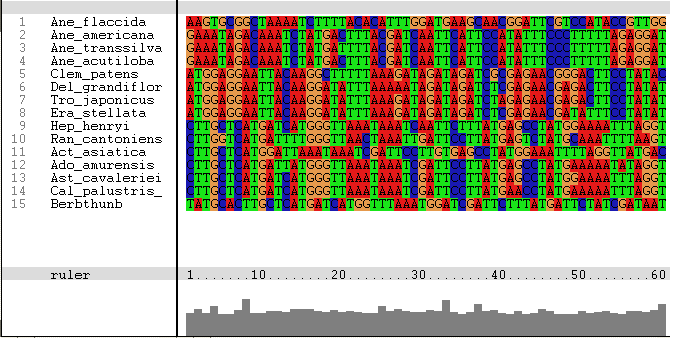
\includegraphics[height=2.5in]{phylo6.png}\\
     \end{center}
     DNA序列在比对前
}

\frame{
    \frametitle{序列比对Alignment}
将DNA序列对齐, 以便寻找突变的位点, 以推断系统发育关系
      \begin{center}
     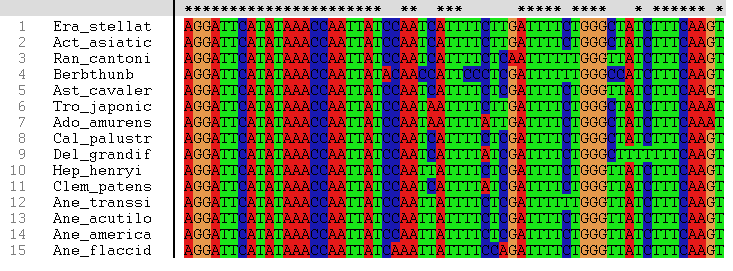
\includegraphics[height=2.in]{phylo7.png}\\
     \end{center}
     DNA序列在比对后
}

\frame{
    \frametitle{序列比对之后的检查和校对}
为什么要检查和校对?
测序的错误, 如ab1峰图文件, 在序列的起始以及结束20bp左右, 质量不佳, 容易误判。 
主要用到的软件: 
\begin{itemize}
\item Bioedit
\item ChromasLite
\item ContigExpress
\item DNAman等
\end{itemize}
}

\frame{
    \frametitle{Bioedit检查和校对比对好的DNA序列}
      \begin{center}
     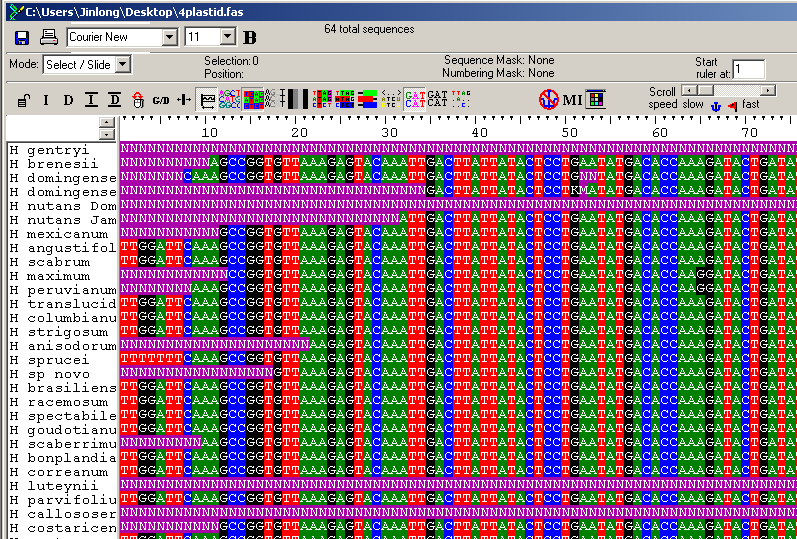
\includegraphics[height=3.in]{phylo8.png}\\
     \end{center}
}

\frame{
    \frametitle{碱基替换模型}
    ATCG之间的替换,发生的概率
$$ Prob [k events] = \frac{{\mu t}^k e^{-\mu t}}{k!}$$

考虑ATCG之间的碱基替换率, 可以写成transition matrix 即 转移概率矩阵。 
}

\frame{
    \frametitle{转移概率矩阵}
      \begin{center}
     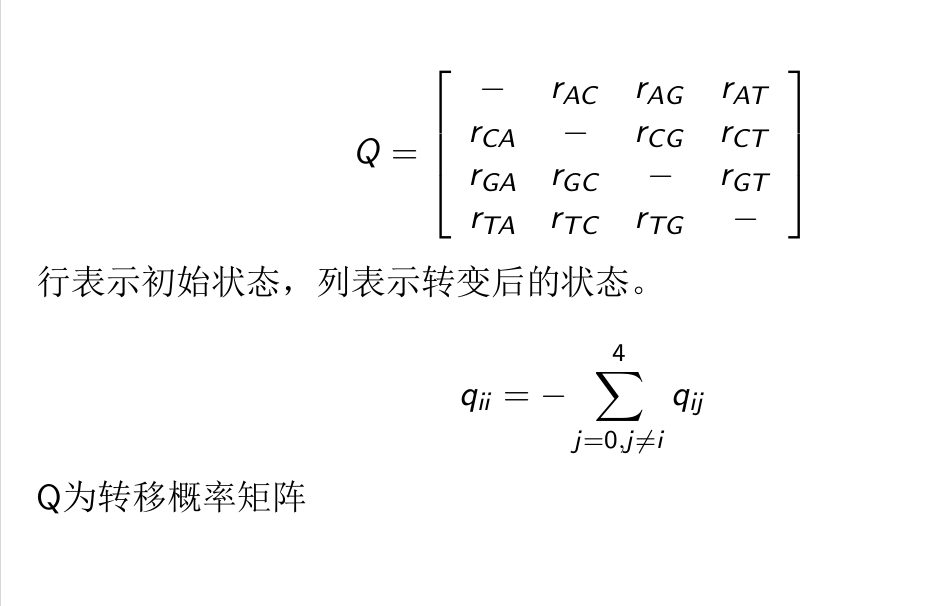
\includegraphics[height=2.5in]{Selection_071.png}\\
     \end{center}
}

\frame{
    \frametitle{JC69模型 Jukes-Cantor 1969}
      \begin{center}
     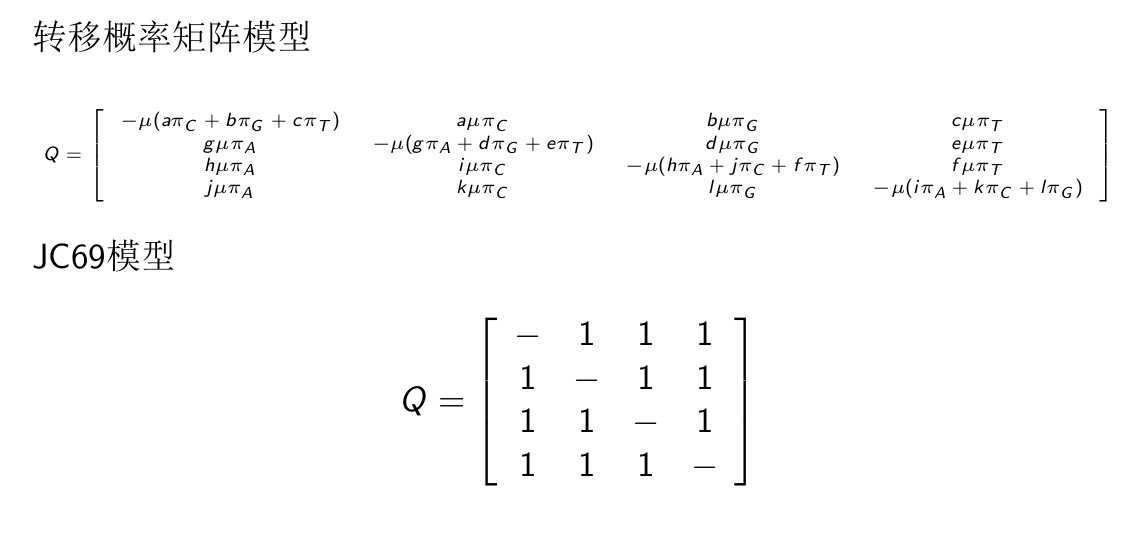
\includegraphics[height=2.1in]{Selection_072.png}\\
     \end{center}
}

\frame{
    \frametitle{Kimura 81模型和F81模型}
      \begin{center}
     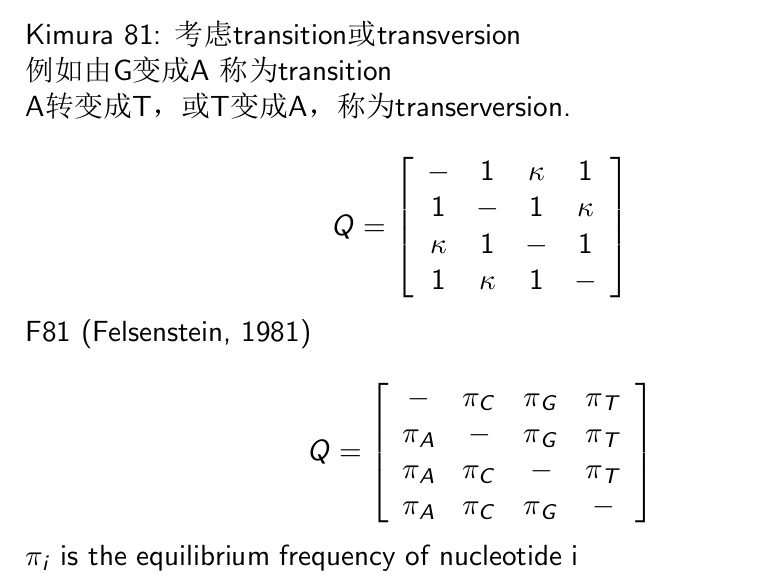
\includegraphics[height=3in]{Selection_073.png}\\
     \end{center}
}

\frame{
    \frametitle{F84模型}
      \begin{center}
     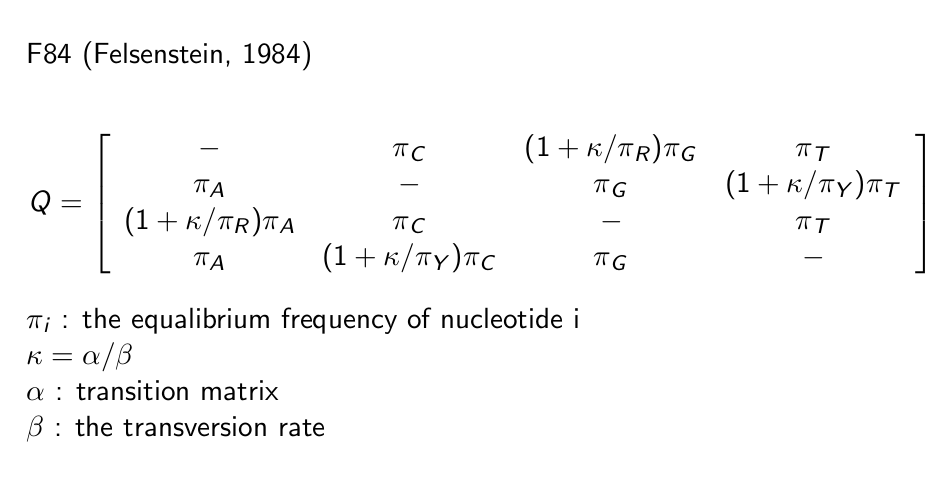
\includegraphics[height=2.5in]{Selection_074.png}\\
     \end{center}
}

\frame{
    \frametitle{HKY85模型和Tamura-Nei93}
      \begin{center}
     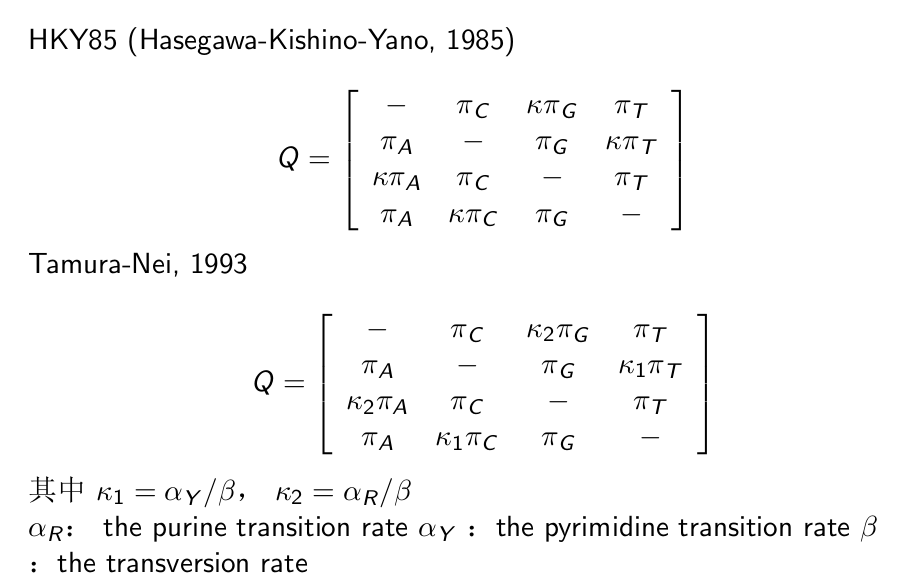
\includegraphics[height=2.5in]{Selection_075.png}\\
     \end{center}
}

\frame{
    \frametitle{HKY85模型和Tamura-Nei93}
      \begin{center}
     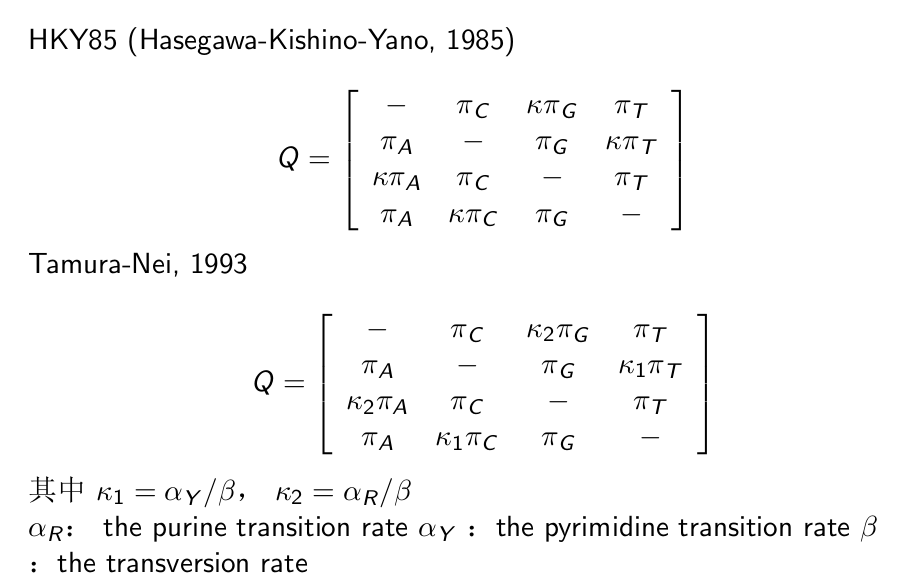
\includegraphics[height=2.5in]{Selection_075.png}\\
     \end{center}
}

\frame{
    \frametitle{GTR: General Time Reversible Model}
      \begin{center}
     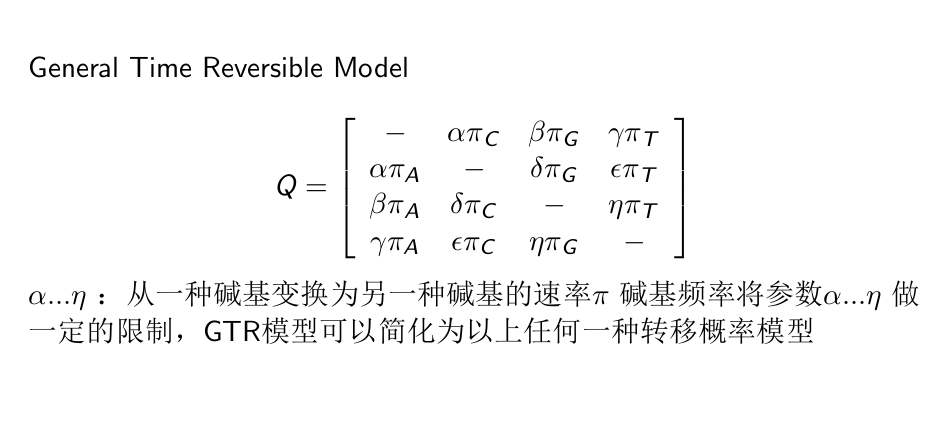
\includegraphics[height=2.in]{Selection_076.png}\\
     \end{center}
}

\frame{
    \frametitle{DNA碱基替换模型之间的关系}
      \begin{center}
     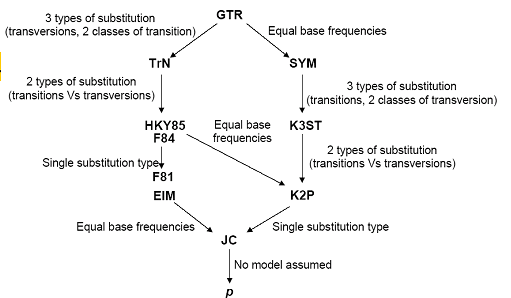
\includegraphics[height=2.5in]{phylo9.png}\\
     \end{center}
}


\frame{
    \frametitle{Gamma 分布拟合不同碱基的不同替换速率}
不同位置的核苷酸具有不同的编译速率,这种变异一般用Gamma分布进行拟合。 \\
}

\frame{
    \frametitle{进化模型的筛选}
模型的筛选: 用 Modeltest, Jmodeltest等, 依据AIC或者LRT进行筛选。\\
如果数据较小, 如出现的信息位点较少, 对于GTR模型+Gamma容易出现模型的过度拟合, 此时就需要进行模型筛选。 对于大数据, 建议用GTR+Gamma。 \\
}


\frame{
    \frametitle{基于遗传距离的建树方法}
    \begin{itemize}
    \item 距离法
    \item 简约法
    \item 极大似然法
    \item 贝叶斯法
    \end{itemize}
}

\frame{
    \frametitle{基于遗传距离的建树方法}
\begin{itemize}
\item 计算序列之间的遗传距离, 基于RAW或者Transition或者Tranversion, 或者其他DNA碱基替换模型。
\item 进行聚类,一般用UPGMA聚类。
\item Neighbour Joining方法
\item Minumum Evolution
\item 基于遗传距离聚类的进化树已经很少使用!
\end{itemize}
}

\frame{
    \frametitle{简约法}
    简约法背后的哲学: 真实的进化历史背后, 所经历的进化事件最少。即碱基突变的位点最少\\
简约法的优点
\begin{itemize}
\item 容易解释
\item 速度快
\item 一般情况下,进化树结构准确。  
\end{itemize}
简约树常用于构建其他进化树的起始树。 
}

\frame{
    \frametitle{极大似然法 1}
    假设已经有一棵进化树T, 以及碱基替换模型Q, 获得当前DNA比对格局的可能性有多大? Likelihood\\
      \begin{center}
     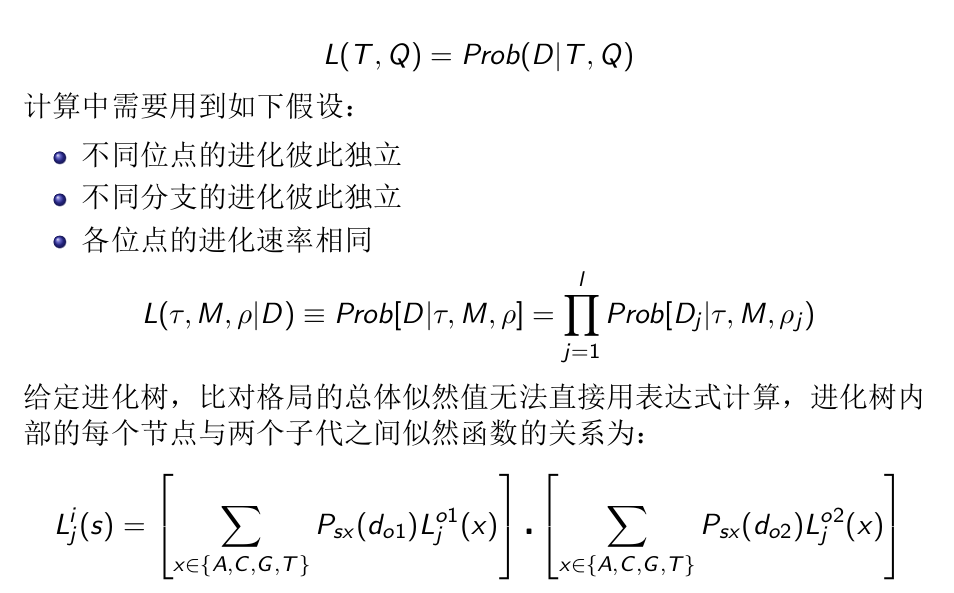
\includegraphics[height=2.5in]{Selection_077.png}\\
     \end{center}
}

\frame{
    \frametitle{极大似然法 2}
      \begin{center}
     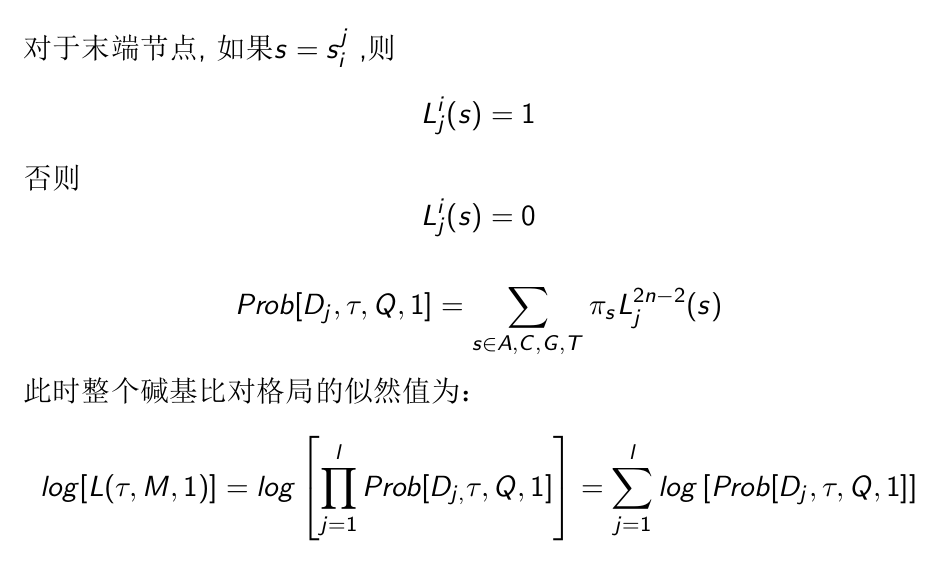
\includegraphics[height=2.5in]{Selection_078.png}\\
     \end{center}
}

\frame{
    \frametitle{为什么构建进化树极为耗时?}
    分类单元数: 可能的进化树的数量\\
 3:     1\\
 5:     15\\
 10:     2027025\\
 15:     7905853580625\\
 16: 213458046676875\\
17: 6190283353629374\\
18: 191898783962510624\\
19: 6332659870762850304\\
20: 2.216430954767e+20\\
30: 8.687364e+36\\
50: 2.838063e+74\\

}

\frame{
    \frametitle{启发式搜索}
从某一个随机的进化树开始,寻找Maximum Likelihood。进行物种逐步添加, 以及进行进化树拓扑结构的变换(剪接和重排) \\
从多个随机的进化树开始, 有助于寻找到全局最优进化树。 \\
}

\frame{
    \frametitle{进化树的剪接和重排}
      \begin{center}
     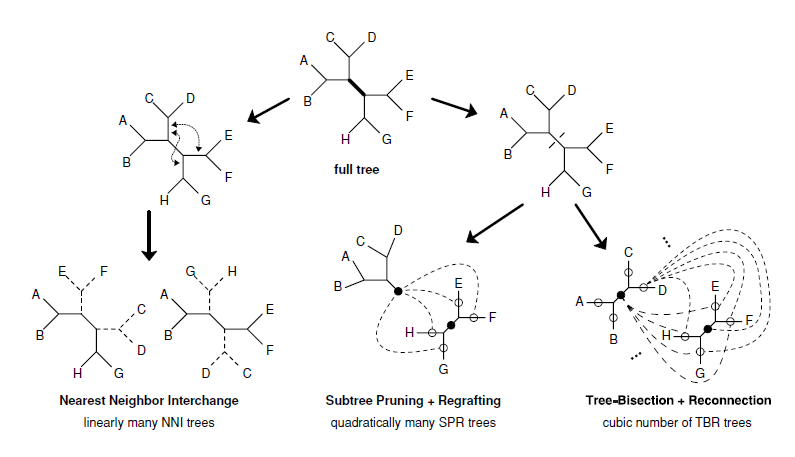
\includegraphics[height=2.5in]{phylo11.png}\\
     \end{center}
}

\frame{
    \frametitle{贪婪算法(Greedy Algorithm)的误区 }
      \begin{center}
     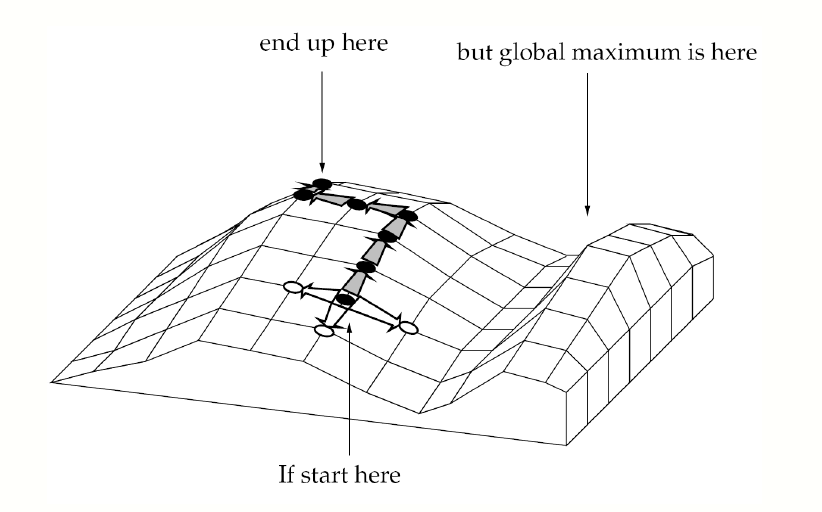
\includegraphics[height=2.5in]{phylo16.png}\\
     \end{center}
     可能滞留在局域最优进化树上
}


\frame{
    \frametitle{基于启发式搜索寻找全局最优树的方法}
\begin{itemize}
\item 进化树合并 Tree fusing
\item 遗传算法 genetic algorithms
\item 进化树局部全搜索 tree windowing
\item 加权搜索 search by reweighting
\item 模拟退火 simulated annealing

\end{itemize}
}


\frame{
    \frametitle{用ML法构建进化树的软件 }
      \begin{center}
     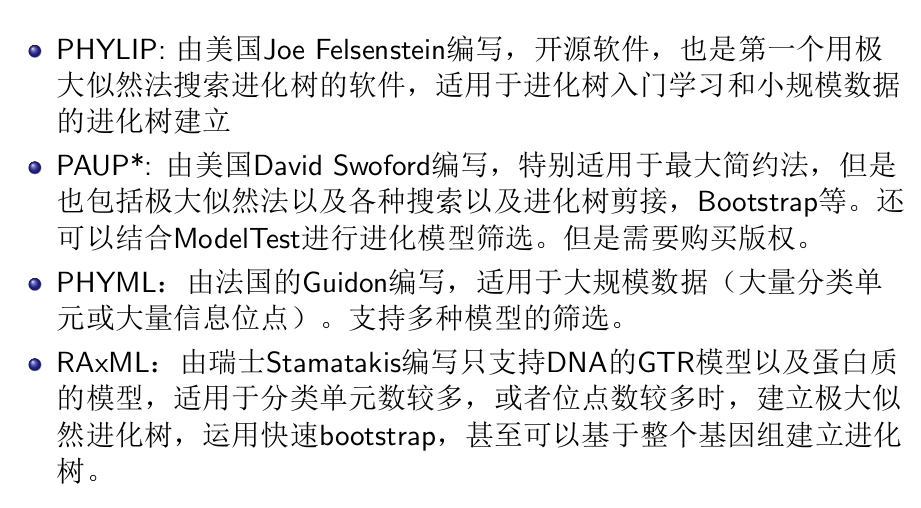
\includegraphics[height=2.2in]{Selection_079.png}\\
     \end{center}
}

\frame{
    \frametitle{进化树的Bootstrap与节点支持率 }
      \begin{center}
     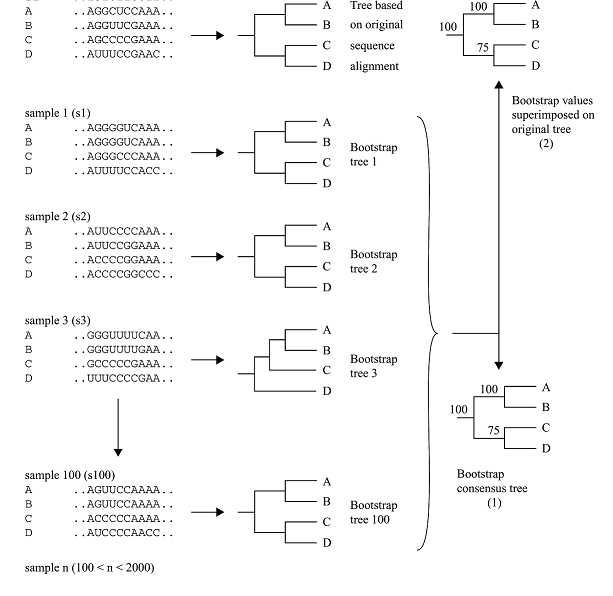
\includegraphics[height=2.5in]{phylo12.png}\\
     \end{center}
}

\frame{
    \frametitle{贝叶斯方法推断进化树}
      \begin{center}
     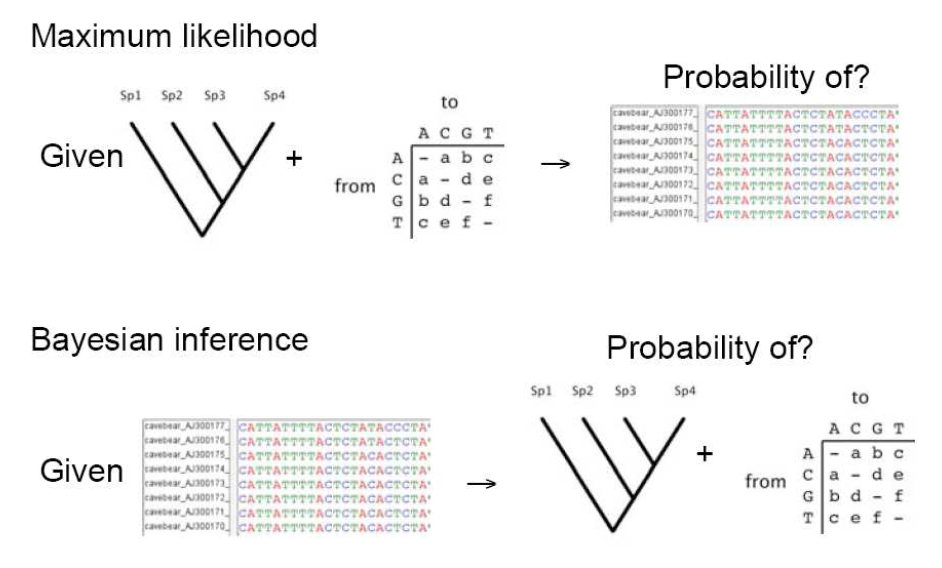
\includegraphics[height=3in]{phylo13.png}\\
     \end{center}
}

\frame{
    \frametitle{贝叶斯方法建树}
      \begin{center}
     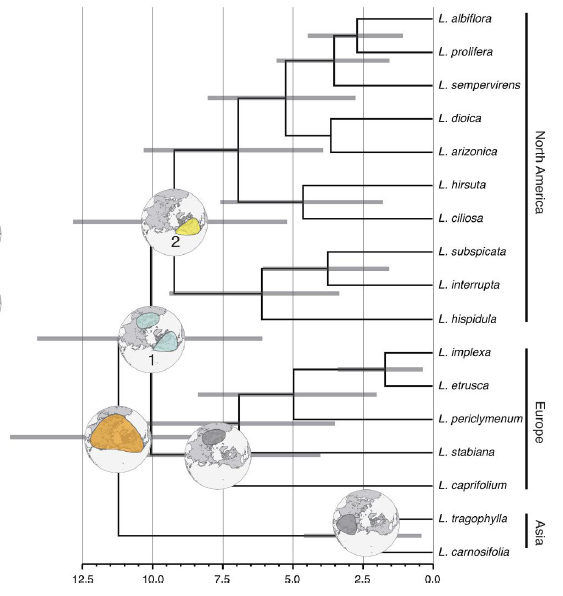
\includegraphics[height=2.5in]{phylo14.png}\\
     \end{center}
     BEAST以及MrBayes是用贝叶斯方法建立进化树的最重要软件。 BEAST建立的进化树同时进行了分子钟校对。
}


\frame{
    \frametitle{分子钟:枝长的意义}
\begin{itemize}
\item 距离法: 枝长表示遗传距离
\item 简约法: 枝长表示发生变异的位点数
\item ML和贝叶斯法: 枝长表示位点的变异。 
\end{itemize}
对于ML进化树来讲, 如果枝长较长,则可能是由于碱基替换速率高, 或者分化的时间足够长。 为了让枝长表示分化时间, 需要进行分子钟校订。
}

\frame{
    \frametitle{分子钟校订的软件}
\begin{itemize}
\item r8s: 非参数速率平滑 NPRS ; 似然罚分法: Penalized Likelihood
\item BEAST: 构建进化树时直接进行了分子钟校订。 
\item ape程序包: PL方法等
\item multidivide time: 基于贝叶斯的方法
\end{itemize}
}

\frame{
    \frametitle{分子钟校订前后}
  \begin{center}
     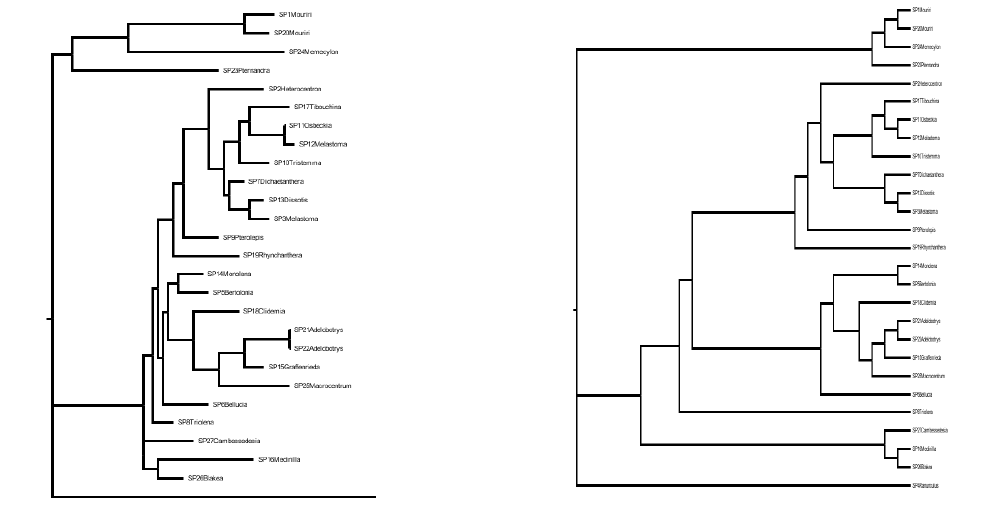
\includegraphics[height=2.5in]{phylo15.png}\\
     \end{center}
     左图:校订之前\\
     右图:校订之后
}

\frame{
    \frametitle{练习}
    \begin{itemize}
    \item 用MUSCLE比对序列\\
    \item 用phylotools转换成Relaxed Phylip\\
    \item 用RAxML构建ML进化树\\
    \item 用Figtree将RAxML Best Tree转换成Nexus格式
    \item 用r8s进行分析钟校订\\
    \end{itemize}
}

\section{系统发育比较分析的核心:APE程序包}
\begin{frame}
\frametitle{目录}
\tableofcontents[currentsection] 
\end{frame}

\frame{
    \frametitle{APE: Analysis of Phylogenetics and Evolution}
    APE 是法国 E. Paradis 等人编写的用于进化分析的程序包\\
http://ape-package.ird.fr/ape\_authors.html\\
该程序包定义了存储进化树信息的phylo类, 成为进行系统发育比较分析的基础。 
    
ape provides functions for:
\begin{itemize}
\item reading and manipulating phylogenetic trees and DNA sequences, 
\item computing DNA distances, 
\item estimating trees with distance-based methods, 
\item a range of methods for comparative analyses and analysis of diversification. 
\item Functionalities are also provided for programming new phylogenetic methods.
\end{itemize}
Paradis, E. (2012) Analysis of Phylogenetics and Evolution with R (Second Edition). New York: Springer.
}

\frame{
    \frametitle{读取进化树 read.tree}
该函数用来读取newick格式的进化树, 并生成phylo类型的对象。 phylo对象的本质是一个列表 list
带有四个向量, 分别为 
edge: 表示分支之间的拓扑关系;
Nnode: 内部的节点数量;
tip.label: 分类单元的名称;
edge.length: 枝长

 \begin{center}
     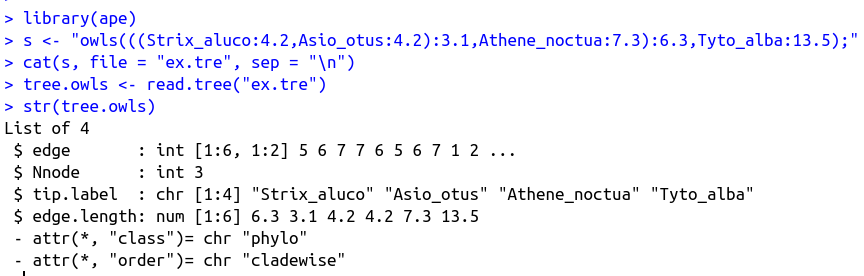
\includegraphics[height=1.8in]{Selection_064.png}\\
     \end{center}
}

\frame{
    \frametitle{绘制进化树 plot.phylo}
由于读取的进化树以phylo的格式保存, 因此, 基于phylo格式开发的plot.phylo函数, 可以用于绘制进化树。 该函数可以直接用 plot()(泛型函数)来调用。
\\
\tt{
\#\# S3 method for class 'phylo'\\
plot(x, type = "phylogram", use.edge.length = TRUE,
    node.pos = NULL, show.tip.label = TRUE, show.node.label = FALSE,
    edge.color = "black", edge.width = 1, edge.lty = 1, font = 3,
    cex = par("cex"), adj = NULL, srt = 0, no.margin = FALSE,
    root.edge = FALSE, label.offset = 0, underscore = FALSE,
    x.lim = NULL, y.lim = NULL, direction = "rightwards",
    lab4ut = NULL, tip.color = "black", plot = TRUE,
    rotate.tree = 0, open.angle = 0, node.depth = 1,
    align.tip.label = FALSE, ...)
}
}

\frame{
    \frametitle{保存绘制的进化树}

\#\#\# An extract from Sibley and Ahlquist (1990)\\
\tt{
tiff(filename = "tree.tiff",
     width = 2400, height = 2400, units = "px", pointsize = 12, res = 600, 
     compression ="lzw") \\

cat("(((Strix\_aluco:4.2,Asio\_otus:4.2):3.1,",
   "Athene\_noctua:7.3):6.3,Tyto\_alba:13.5);",
   file = "ex.tre", sep = "\\n") \\
tree.owls $<-$ read.tree("ex.tre") \\
plot(tree.owls) \\
dev.off() \\
}
}


\frame{
\frametitle{ape中的重要函数 I}

\begin{itemize}
\item ace()	Ancestral Character Estimation
\item ladderize()	Ladderize a Tree
\item bd.ext()	Extended Version of the Birth-Death Models to Estimate Speciation and Extinction Rates
\item chronopl()	Molecular Dating With Penalized Likelihood
\item consensus()	Concensus Trees
\item di2multi()	Collapse and Resolve Multichotomies
\item drop.tip()	Remove Tips in a Phylogenetic Tree
\end{itemize}

}

\frame{
\frametitle{ape中的重要函数 II}

\begin{itemize}
\item gammaStat()	Gamma-Statistic of Pybus and Harvey
\item ladderize()	Ladderize a Tree
\item ltt.plot()	Lineages Through Time Plot
\item mrca()	Find Most Recent Common Ancestors Between Pairs
\item multi2di()	Collapse and Resolve Multichotomies
\item read.nexus()	Read Tree File in Nexus Format
\item root()	Roots Phylogenetic Trees
\item rtree()	Generates Random Trees
\item write.nexus()	Write Tree File in Nexus Format
\item write.tree()	Write Tree File in Parenthetic Format
\end{itemize}

}



%%########################

\frame{
\frametitle{ggtree是绘制进化树的程序包}
ggtree是香港大学公共卫生学院在读博士生余光创先生编写的R程序包。ggtree将进化树看做点拓扑关系的集合, 绘制进化树的线段是后期处理获得。 ggtree是ggplot2程序包的良好扩展, 能够很好得用图层方式的语法对对象修改, 因此, 通过较为简单的参数, 即可完成十分复杂的进化树绘制。 

ggtree提供了多种进化树格式的读取, 并且能够读取并转换BEAST, r8s,RAxML等软件所生成的数据。用于也可自定义数据, 轻松实现R实现基于进化树的高级绘图。 
 \begin{center}
     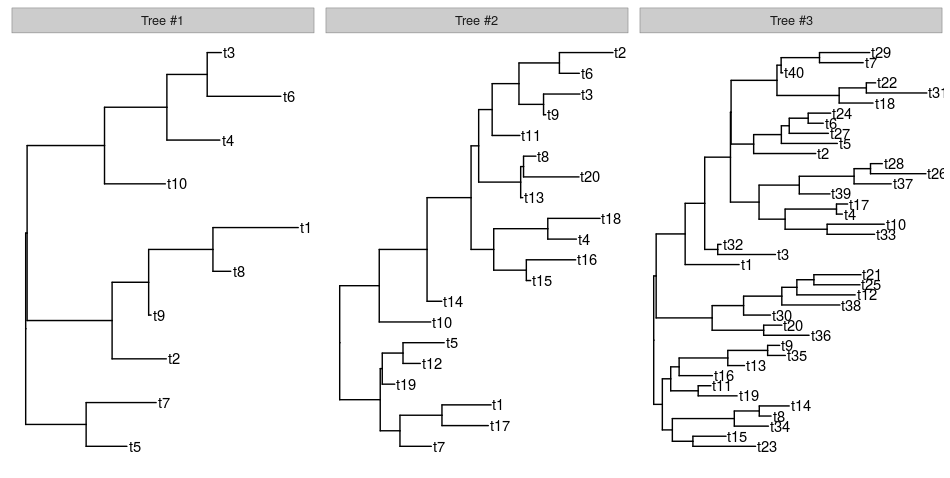
\includegraphics[height=1.in]{Rplot05.png}\\
     \end{center}
}


\frame{
\frametitle{ggtree 举例}
\tt{
trees <- lapply(c(10, 20, 40), rtree) \\
class(trees) <- "multiPhylo" \\
ggtree(trees) + facet\_wrap(\~.id, scale="free") + geom\_tiplab() \\
可参考 http://blog.sciencenet.cn/home.php?mod=\\
space\&uid=255662\&do=blog\&id=969228
}
}

\section{物种形成和灭绝速率的估计}
\begin{frame}
\frametitle{目录}
\tableofcontents[currentsection] 
\end{frame}


\frame{
\frametitle{Lineages Through Time Plot}
ltt plot
 \begin{center}
     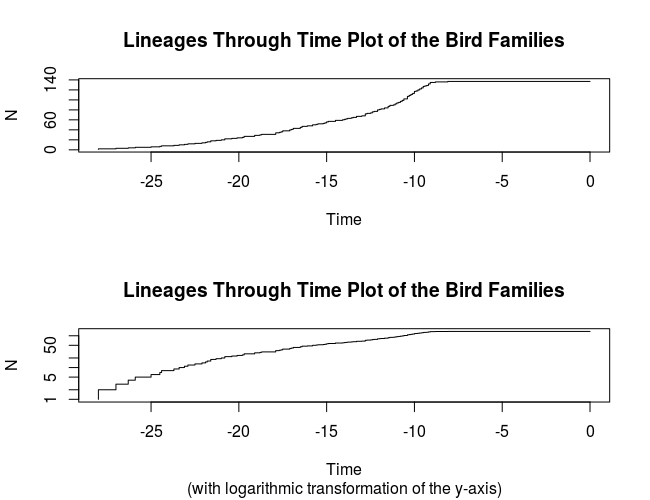
\includegraphics[height=3in]{Rplot.png}\\
     \end{center}
}


\frame{
\frametitle{Laser:基于ltt plot估计 物种形成和灭绝速率}

Laser 程序包由 Dan Rabosky开发。 是用极大似然法进行物种形成和灭绝速率进行估计。\\
包括三种模型:\\
1. 物种形成速率随时间的变化而降低, 但灭绝速率恒定 (SPVAR)\\
2. 物种形成速率恒定, 但是物种灭绝速率随时间上升 (EXVAR)\\
3. 物种形成随时间下降, 同时物种的灭绝速率上升 (BOTHVAR)\\
}

\frame{
\frametitle{Laser: Likelihood Analysis of Speciation/Extinction Rates from Phylogenies}
 \begin{center}
     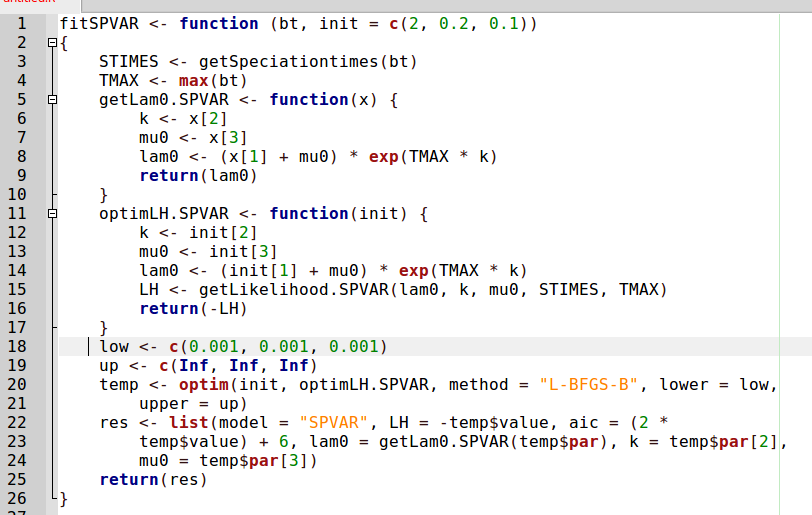
\includegraphics[height=2.5in]{Selection_068.png}\\
     \end{center}
}

\frame{
\frametitle{Geiger分析物种分化速率 MEDUSA}
Modeling Evolutionary Diversification Using Stepwise AIC
 \begin{center}
     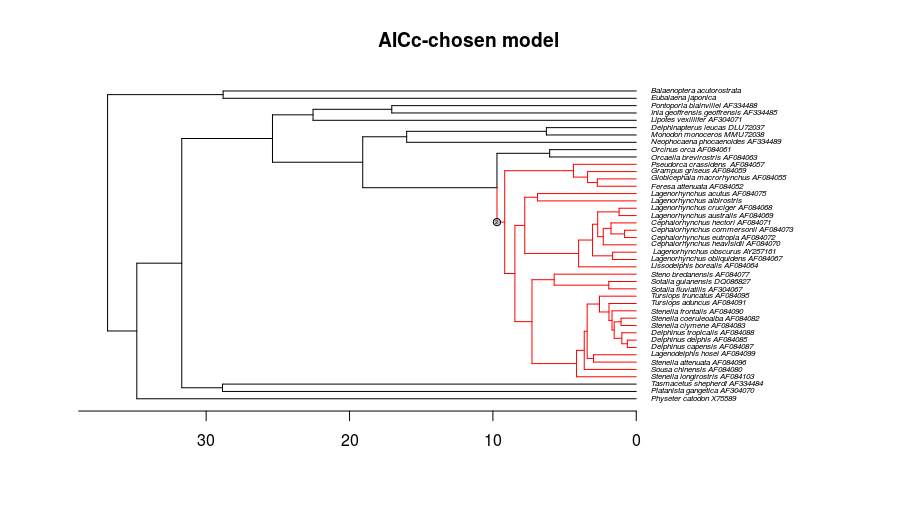
\includegraphics[height=2.5in]{Rplot02.png}\\
     \end{center}
geiger::medusa
}


\frame{
\frametitle{diversitree 安装}

\begin{center}
     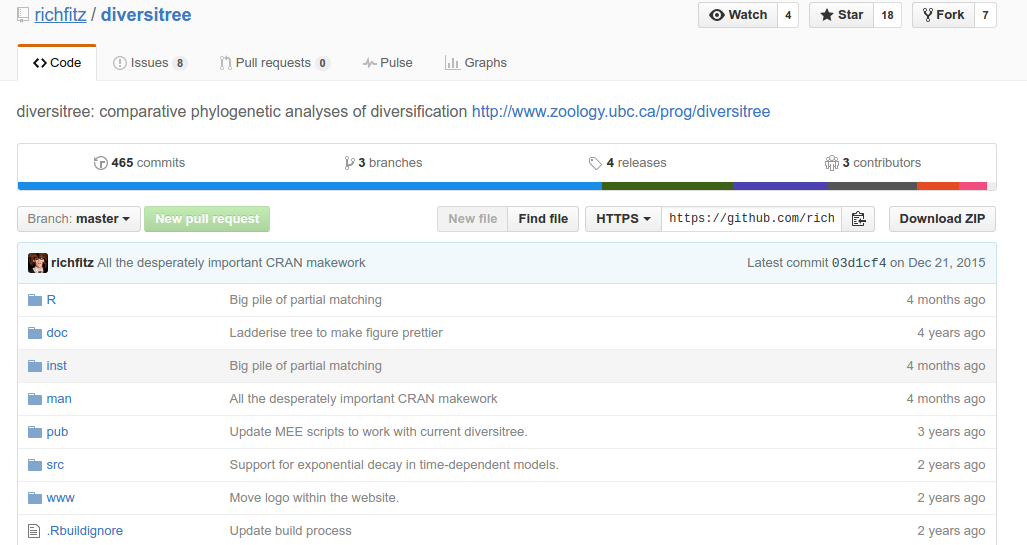
\includegraphics[height=2.5in]{Selection_065.png}\\
 \end{center}
 install.packages(''diversitree'')
}

\frame{
\frametitle{diversitree}

\begin{center}
     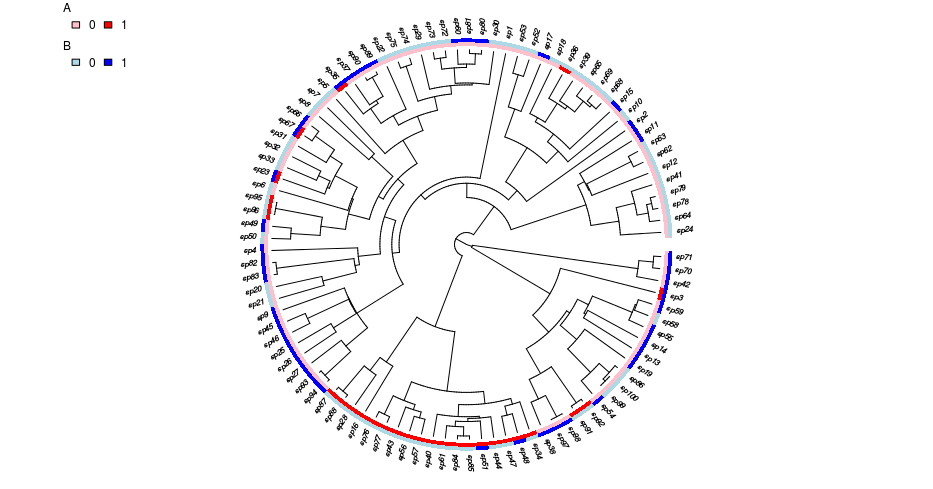
\includegraphics[height=2in]{Rplot03.png}\\
 \end{center}
}


\frame{
\frametitle{重建祖先状态 Ancestral Character Estimation}

\begin{center}
     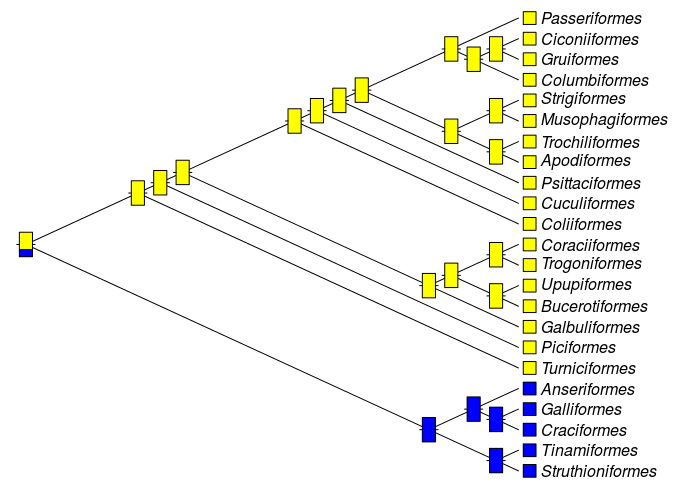
\includegraphics[height=2in]{Rplot04.png}\\
 \end{center}
 ape::ace
}

\section{系统发育多样性}
\begin{frame}
\frametitle{目录}
\tableofcontents[currentsection] 
\end{frame}


\frame{
\frametitle{系统发育多样性}
\begin{itemize}
\item Faith's PD Phylogenetic Diversity (Faith 1992) 连接某地点所有出现物种的枝长总和。 picante::pd()
\item 系统发育信号(Blomberg's K): 检验系统发育相近的分类单元是否具有相近的性状。picante::phylosignal() 

\item 进化的独特性 Evolutionary Distinctiveness: 每个进化树中, 每个分类单元所独占的系统发育信息。 picante::evol.distinct()
\end{itemize}

}

\frame{
    \frametitle{系统发育beta多样性}
    系统发育beta多样性: Phylogenetic Beta diversity\\
系统发育beta多样性是群落或地点之间系统发育距离的度量(Fine and Kembel 2010)\\
\begin{tabular}{ll}
{\color{blue}\textbf{comdist()\& comdistnn()}}&:MPD和MNTD (Webb 2000)\\
{\color{blue}\textbf{phylosor()}}&:Phylosor (Bryant et al. 2008)\\
{\color{blue}\textbf{unifrac():  }}&:Unifrac(Lozupone et al. 2006)\\
{\color{blue}\textbf{rao()}}&:Rao 1982, Jost 2007, Webb et al. 2008\\
{\color{blue}\textbf{pcd()}}&:PCD (Ives and Helmus 2010)\\
\end{tabular}
}
\frame{
    \frametitle{群落系统结构中的零模型 Null Models}
群落系统发育分析中零模型,是将群落内物种组成的关系进行随机化的一系列方法。按照中性理论,物种与物种之间是等同的, 因此,群落中物种应该是随机组合的。\\
群落系统发育分析中,一般通过以下四种方式进行随机化。\\
\begin{itemize}
\item Null 0 群落数据不变,但是物种在进化树末端随机排列。\\
\item Null 1 进化树不变,物种在样方中随机排列,物种从所有样方中随机选取。\\
\item Null 2 进化树不变,物种在样方中随机排列,物种从指定的物种库中选取。\\
\item Null 3 进化树不变,与此同时,物种在样方中成对的关系保持不变。这种随机化的方法称为独立交换法(Independent swap)。 \\
\end{itemize}
}


\section{植物学名的处理以及科属查询}
\begin{frame}
\frametitle{目录}
\tableofcontents[currentsection] 
\end{frame}


\frame{
\frametitle{分类位置查询}
程序包主要为 taxize, taxonstand, plantlist
\begin{itemize}
\item status(): Looking for the taxonomic status of species
\item data(acc\_dat): The accepted plant names from the Plant List
\item data(syn\_dat): Synonyms database from The Plant List
\item taxa.table(): Making a Taxa Table based on the result of function TPL for Phylomatic
\item TPL(): Looking up Family, Family Number and Order in Modern Classification Systems.
\end{itemize}
}

\frame{
\frametitle{用plantlist程序包查询植物科属}

\begin{center}
     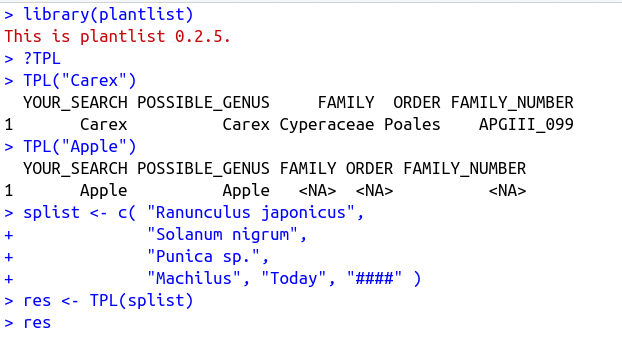
\includegraphics[height=2in]{Selection_069.png}\\
 \end{center}
 plantlist::TPL
}


\frame{
\frametitle{参考材料}
https://cran.r-project.org/web/views/Phylogenetics.html

}

\frame{
    \begin{center}
    \Large {\color{blue} 
     问题?\\
    } 
    \end{center}
}


\frame{
    \begin{center}
    \Large {\color{blue} 
      谢谢!\\
      敬请批评指正\\
    } 
    \end{center}
}

\end{document}
